\Aufgabe{Spiel-Vorlage und erster Start}

\begin{itemize}
    \item Kopiere den \textbf{ganzen Ordner} SpielProjekt vom Ressourcen-Laufwerk in euren Ordner H:\\  \emph{R:/gy0187/klassen/gy0187-klasse-9b/Vorlagen/SpielProjekt}
    \item Öffne die Datei \emph{package.bluej} (manchmal heißt sie auch nur \emph{package}) in deiner Kopie der Vorlage.
    \item War das erfolgreich, kannst du ein Spielfeld-Objekt und ein Spieler-Objekt erstellen, das Spielerobjekt zum Spielfeld hinzufügen und das Spiel starten (siehe Bilder unten).
\end{itemize}

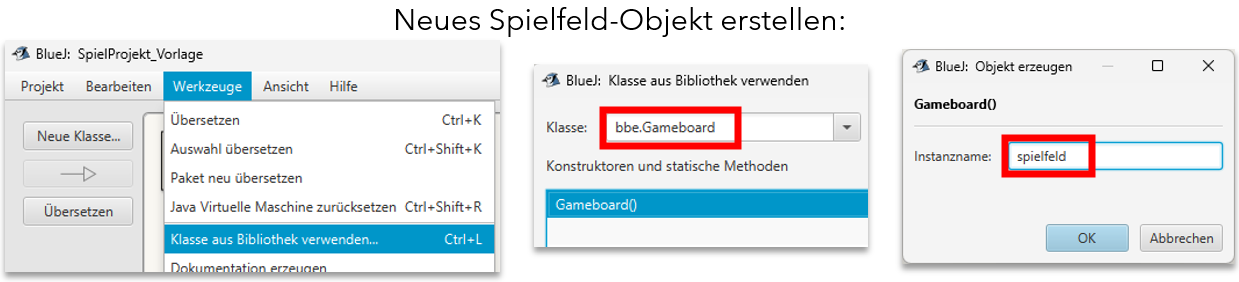
\includegraphics[width =\textwidth]{_Aufgaben/BlocklyJava_Skript/img/A10_CreateGB.png}

\vspace{0.2cm}
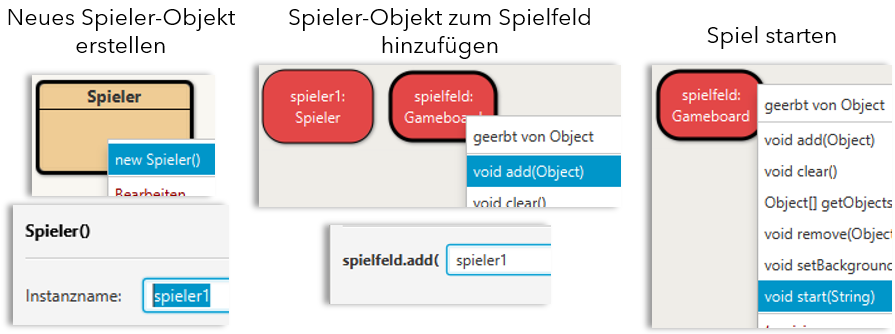
\includegraphics[width=\textwidth]{_Aufgaben/BlocklyJava_Skript/img/A10_StartGame.png}
